\section{Keylengths}
\label{section:keylengths}


\epigraph{``On the choice between AES256 and AES128: I would never consider
using AES256, just like I don't wear a helmet when I sit inside my car. It's
too much bother for the epsilon improvement in security.''}{-- Vincent Rijmen
in a personal mail exchange Dec 2013}

Recommendations on keylengths need to be adapted regularly. Since this document
first of all is static and second of all, does not consider itself to be
authoritative on keylengths, we would rather refer to existing publications and
websites.  Recommending a safe key length is a hit-and-miss issue.

Furthermore, when choosing an encryption algorithm and keylength, the
designer/sysadmin always needs to consider the value of the information and how
long it must be protected.  In other words: consider the number of years the
data needs to stay confidential.


The ECRYPT II publication (\cite{ii2011ecrypt}) gives a fascinating overview of
strengths of symmetric keys in chapter 5 and chapter 7. Summarizing ECRYPT II, we
recommend 128 bit of key strength for symmetric keys. In ECRYPT II, this is
considered safe for security level 7, long term protection.

In the same ECRYPT II publication you can find a practical comparison of key size
equivalence between symmetric key sizes and RSA, discrete log (DLOG) and EC
keylengths. ECRYPT II arrives at the interesting conclusion that for an
equivalence of 128 bit symmetric size, you will need to use an 3248 bit RSA
key. See chapter 7 of \cite{ii2011ecrypt}, page 30.


There are a couple of other studies comparing keylengths and their respective
strengths.  The website \url{http://www.keylength.com/} compares these papers
and offers a good overview of approximations for key lengths based on
recommendations by different standardization bodies and academic publications.
Figure \ref{fig:keylengths.com} shows a typical comparison of keylengths on
this web site.

\begin{figure}[h]
  \centering
  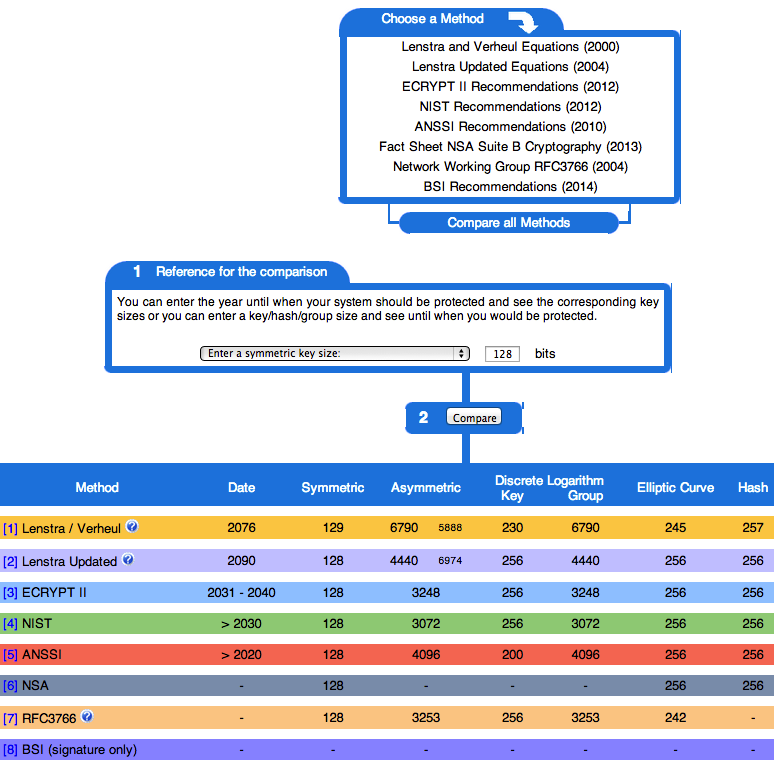
\includegraphics[width=0.65\textwidth]{img/keylengths_com.png}
  \caption{Screenshot of \url{http://www.keylength.com} for 128 bit symmetric key size equivalents}
  \label{fig:keylengths.com}
\end{figure}


\paragraph{Summary}
\begin{itemize}

\item For traditional asymmetric public-key cryptography we consider any key
length below 2048 bits to be deprecated at the time of this writing (for long
term protection).  

\item For elliptic curve cryptography we consider key lengths below 256 bits to
be inadequate for long term protection.  

\item For symmetric algorithms we consider anything below 128 bits to be
inadequate for long term protection.

\end{itemize}

\paragraph{Special remark on 3DES} \mbox{} \\
We want to note that 3DES theoretically has 168 bits of security, however based
on the NIST Special Publication 800-57
\footnote{\url{http://csrc.nist.gov/publications/PubsSPs.html\#800-57-part1},
pages 63 and 64}, it is clear that 3DES can only be considered to provide for
80 bits / 112 bits security.





